\documentclass[12pt,twocolumn]{article}

\usepackage{sbc-template}
\usepackage[utf8]{inputenc}
\usepackage[brazil]{babel}
\usepackage{graphicx}
\usepackage{url}
\usepackage{booktabs}
\usepackage{amsmath}
\usepackage{amssymb}
\usepackage{float}
\usepackage{microtype}
\usepackage{caption}
\captionsetup{font=small, labelfont=bf}

% \graphicspath{{figuras/}}  % remova o comentário se compilar localmente

\title{Desenvolvimento e Avaliação Experimental de uma\\
       Ferramenta Genérica para Algoritmos Genéticos}

\author{Andre Fidelis Jr.}
\address{Disciplina de Tópicos Especiais em Inteligência Computacional\\
         Universidade do Estado de Santa Catarina (UDESC) --- Joinville/SC}

\begin{document}
\maketitle

\begin{resumo}
Este trabalho apresenta o desenvolvimento de uma ferramenta genérica para execução de
Algoritmos Genéticos, implementada em Python. A ferramenta permite configurar parâmetros
evolutivos, diferentes representações de cromossomos e funções de \textit{fitness}
específicas para cada problema. Foram realizados experimentos com três problemas:
otimização de uma função matemática (maximização e minimização), problema dos rádios com
restrição e uma instância 3-SAT. Para cada problema, foram realizadas 10~execuções
independentes. Os resultados indicam alta consistência entre as execuções e demonstram a
capacidade da ferramenta de produzir soluções de qualidade em domínios distintos.
\end{resumo}

% ------------------------------------------------------------------
\section{Introdução}
% ------------------------------------------------------------------

A Computação Evolutiva compreende uma família de técnicas inspiradas em processos naturais
de evolução, adaptação e seleção. Nesse paradigma, o problema atua como o ambiente,
enquanto cada indivíduo representa uma possível solução; quanto melhor a solução, maior
sua aptidão ou \textit{fitness}~\cite{vonzuben2000}.

Entre as principais técnicas de Computação Evolutiva estão os Algoritmos Genéticos
(AGs), que mantêm uma população de indivíduos, avaliam cada um por meio de uma função
\textit{fitness} e aplicam operadores genéticos para gerar novas soluções. Indivíduos
mais adaptados possuem maior probabilidade de participar da geração seguinte, embora
elementos aleatórios sejam mantidos para preservar diversidade e explorar o espaço de
busca~\cite{tutorialspoint2016}.

A motivação para o uso de AGs está relacionada à sua capacidade de atuar como métodos
gerais de busca e otimização. Eles são especialmente úteis em problemas com espaço de
busca elevado, funções objetivo não lineares, multimodais, não diferenciáveis ou difíceis
de resolver por métodos exatos. Apesar de não garantirem a solução ótima global, podem
produzir soluções boas ou próximas do ótimo em tempo computacional aceitável.

Este trabalho tem como objetivo o desenvolvimento e a avaliação experimental de uma
ferramenta genérica para AGs implementada em Python. A ferramenta é aplicada a três
problemas: (i)~maximização e minimização de uma função matemática; (ii)~problema dos
rádios com restrição por penalização; e (iii)~instância do problema 3-SAT.

O texto está organizado da seguinte forma: a Seção~2 apresenta a metodologia de
desenvolvimento; a Seção~3, os experimentos e resultados; a Seção~4, a análise dos
resultados; e a Seção~5, as conclusões.

% ------------------------------------------------------------------
\section{Metodologia de Desenvolvimento}
% ------------------------------------------------------------------

A ferramenta foi desenvolvida em Python com o objetivo de fornecer uma estrutura
genérica para a execução de AGs. A implementação separa claramente o \textit{núcleo
evolutivo} --- contido no módulo \texttt{ae.py} --- das \textit{funções de fitness}
específicas de cada problema.

\subsection{Representação e Estruturas de Dados}

Cada indivíduo (\texttt{Individuo}) possui um cromossomo (\texttt{Cromossomo}) e um valor
de \textit{fitness}. O cromossomo suporta quatro codificações: binária (\texttt{BIN}),
inteira (\texttt{INT}), permutação (\texttt{INT\_PERM}) e real (\texttt{REAL}). Os três
experimentos deste trabalho utilizam exclusivamente a codificação binária.

Os parâmetros do algoritmo são definidos em arquivos JSON, contendo: tipo de codificação,
tamanho da população, dimensão do cromossomo, número de gerações, número de execuções
independentes, limites do domínio, probabilidade de \textit{crossover}, probabilidade de
mutação, tipo de \textit{crossover} e ativação do elitismo. Essa abordagem orientada a
configuração permite trocar os parâmetros sem alterar o código-fonte.

\subsection{Decodificação Binária}

A decodificação de um cromossomo binário de $L$ bits para um valor real no domínio
$[x_{\min}, x_{\max}]$ ocorre em duas etapas. Primeiro, os bits são convertidos para
um inteiro decimal:

\begin{equation}
  d = \sum_{i=0}^{L-1} b_i \cdot 2^i
  \label{eq:bin2dec}
\end{equation}

Em seguida, $d$ é mapeado para o intervalo real por ajuste de escala:

\begin{equation}
  x = x_{\min} + \frac{x_{\max} - x_{\min}}{2^L - 1} \cdot d
  \label{eq:scale}
\end{equation}

\subsection{Ciclo Evolutivo}

Para cada execução independente, o ciclo evolutivo segue as etapas descritas a seguir.

\textbf{Inicialização.} A população inicial $P(0)$ é gerada de forma aleatória uniforme,
com $N$ indivíduos de $L$ bits cada. Para a codificação binária, cada bit recebe valor~0
ou~1 com probabilidade igual a 0,5.

\textbf{Avaliação.} Todos os indivíduos são avaliados pela função de \textit{fitness}
específica do problema. O \textit{fitness} é um valor real positivo que a ferramenta
sempre maximiza, independentemente de o problema original ser de maximização ou
minimização.

\textbf{Seleção.} A seleção é realizada por roleta sem reposição. Cada indivíduo recebe
um peso proporcional ao seu valor de \textit{fitness}:

\begin{equation}
  w_i = \begin{cases}
    f_i - f_{\min} + \varepsilon & \text{se } f_{\min} \le 0 \\
    f_i + \varepsilon & \text{caso contrário}
  \end{cases}
  \label{eq:roleta}
\end{equation}

\noindent onde $\varepsilon = 10^{-9}$ evita pesos nulos. A cada rodada, dois indivíduos
distintos são selecionados, formando a população intermediária.

\textbf{\textit{Crossover}.} Para cromossomos binários, a ferramenta implementa três
operadores: (i)~\textbf{um ponto}: um ponto de corte aleatório divide os pais; os filhos
recebem as metades trocadas; (ii)~\textbf{dois pontos}: um segmento intermediário é
trocado entre os pais; (iii)~\textbf{uniforme}: cada gene do filho é escolhido
independentemente de um dos pais com probabilidade~0,5. Para cromossomos permutacionais,
implementa-se \textit{Cycle Crossover} (CX) e \textit{Partially Mapped Crossover} (PMX).

\textbf{Mutação.} A mutação binária é realizada por \textit{bit flip}: cada bit do
cromossomo é invertido com probabilidade $p_m$. Para permutações, aplica-se a mutação por
troca (\textit{swap}), que seleciona dois genes aleatórios e os permuta.

\textbf{Elitismo.} Quando ativado, o melhor indivíduo da geração atual (elite) é
preservado: antes de qualquer operação genética, o elite é armazenado; após a avaliação
da nova população, ele substitui o pior indivíduo da geração seguinte. Isso garante que o
melhor \textit{fitness} nunca decresce entre gerações.

% ------------------------------------------------------------------
\section{Descrição dos Experimentos e Resultados}
% ------------------------------------------------------------------

Para cada problema, foram realizadas 10~execuções independentes com os mesmos parâmetros,
a fim de avaliar a estabilidade do algoritmo diante de sua natureza estocástica.

\subsection{Experimento 1: Função Matemática}

O primeiro experimento consiste na otimização da função:

\begin{equation}
  f(x) = \cos(20x) - \frac{|x|}{2} + \frac{x^3}{4},
  \quad x \in [-2,\, +2]
  \label{eq:fx}
\end{equation}

\noindent considerando separadamente a maximização e a minimização de $f(x)$.

\textbf{Representação.} Cada cromossomo é uma sequência de $L = 16$ bits. A decodificação
converte os bits para um valor real $x \in [-2, +2]$ pelas Equações~\ref{eq:bin2dec}
e~\ref{eq:scale}. Com 16~bits, obtêm-se $2^{16} = 65\,536$ valores distintos no domínio,
resultando em uma precisão de $\approx 6{,}1 \times 10^{-5}$ por incremento.

\textbf{Função de \textit{fitness}.} Para a maximização, a função de \textit{fitness} é
definida de modo que todos os valores sejam positivos:

\begin{equation}
  \mathit{fit}_{\max} = 4 + f(x)
  \label{eq:fitmax}
\end{equation}

Para a minimização, o problema é convertido em maximização pela inversão:

\begin{equation}
  \mathit{fit}_{\min} = 2 - f(x)
  \label{eq:fitmin}
\end{equation}

As constantes 4 e 2 foram escolhidas de modo a garantir que o \textit{fitness} seja
sempre positivo em todo o domínio $[-2, 2]$, requisito da seleção proporcional.

\textbf{Configuração.} Parâmetros: $N = 10$ indivíduos, $G = 150$ gerações, $p_c = 0{,}8$,
$p_m = 0{,}05$, \textit{crossover} de um ponto e elitismo ativado.

\textbf{Resultados --- Maximização.}
A Tabela~\ref{tab:ex1max} apresenta os resultados das 10~execuções para a maximização
de $f(x)$.

\begin{table}[H]
\centering
\caption{Resultados da maximização de $f(x)$ (10 execuções).}
\label{tab:ex1max}
\small
\begin{tabular}{@{}crrrr@{}}
\toprule
Exec. & $x$ & $f(x)$ & \textit{Fitness} \\
\midrule
1  & 1,890440 &  1,737767 & 5,737767 \\
2  & 1,890440 &  1,737767 & 5,737767 \\
3  & 1,890684 &  1,737753 & 5,737753 \\
4  & 1,890684 &  1,737753 & 5,737753 \\
5  & 1,890684 &  1,737753 & 5,737753 \\
6  & 1,890440 &  1,737767 & 5,737767 \\
7  & 1,890440 &  1,737767 & 5,737767 \\
8  & 1,890684 &  1,737753 & 5,737753 \\
9  & 1,890684 &  1,737753 & 5,737753 \\
10 & 1,890745 &  1,737745 & 5,737745 \\
\midrule
\multicolumn{2}{l}{\textbf{Média}} & 1,737758 & 5,737758 \\
\multicolumn{2}{l}{\textbf{Desv. Pad.}} & 0,000008 & 0,000008 \\
\bottomrule
\end{tabular}
\end{table}

\textbf{Resultados --- Minimização.}
A Tabela~\ref{tab:ex1min} apresenta os resultados para a minimização de $f(x)$.

\begin{table}[H]
\centering
\caption{Resultados da minimização de $f(x)$ (10 execuções).}
\label{tab:ex1min}
\small
\begin{tabular}{@{}crrrr@{}}
\toprule
Exec. & $x$ & $f(x)$ & \textit{Fitness} \\
\midrule
1  & $-$2,000000 & $-$3,666938 & 5,666938 \\
2  & $-$2,000000 & $-$3,666938 & 5,666938 \\
3  & $-$2,000000 & $-$3,666938 & 5,666938 \\
4  & $-$2,000000 & $-$3,666938 & 5,666938 \\
5  & $-$2,000000 & $-$3,666938 & 5,666938 \\
6  & $-$2,000000 & $-$3,666938 & 5,666938 \\
7  & $-$2,000000 & $-$3,666938 & 5,666938 \\
8  & $-$2,000000 & $-$3,666938 & 5,666938 \\
9  & $-$2,000000 & $-$3,666938 & 5,666938 \\
10 & $-$2,000000 & $-$3,666938 & 5,666938 \\
\midrule
\multicolumn{2}{l}{\textbf{Média}} & $-$3,666938 & 5,666938 \\
\multicolumn{2}{l}{\textbf{Desv. Pad.}} & 0,000000 & 0,000000 \\
\bottomrule
\end{tabular}
\end{table}

As curvas de convergência das 10~execuções para maximização e minimização são
apresentadas nas Figuras~\ref{fig:ex1max} e~\ref{fig:ex1min}, respectivamente. Em cada
gráfico, as linhas finas representam as execuções individuais e as linhas espessas
representam a média entre todas as execuções.

\begin{figure}[H]
  \centering
  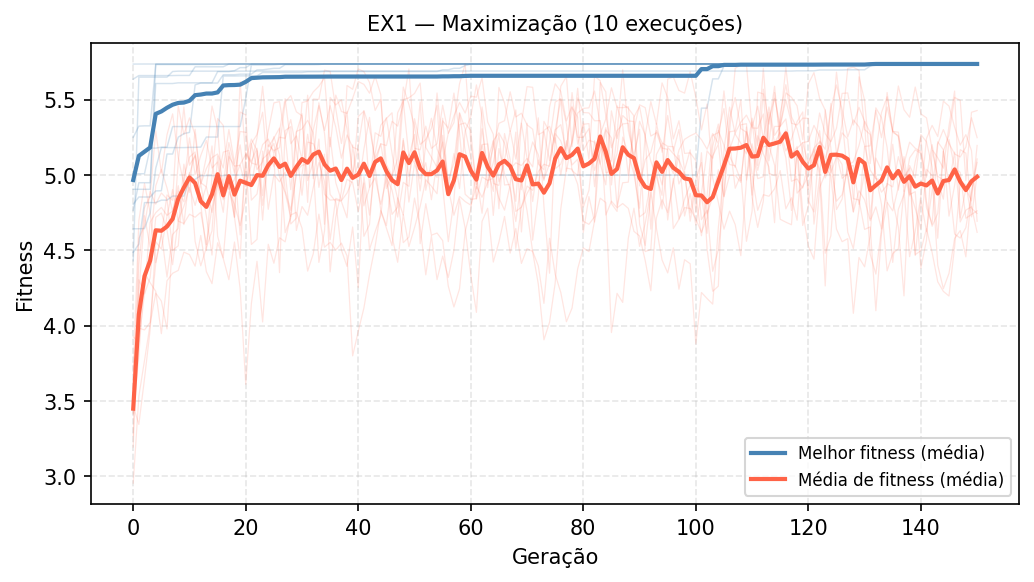
\includegraphics[width=\columnwidth]{ex1_max_conv.png}
  \caption{Convergência do EX1 --- Maximização (10 execuções).}
  \label{fig:ex1max}
\end{figure}

\begin{figure}[H]
  \centering
  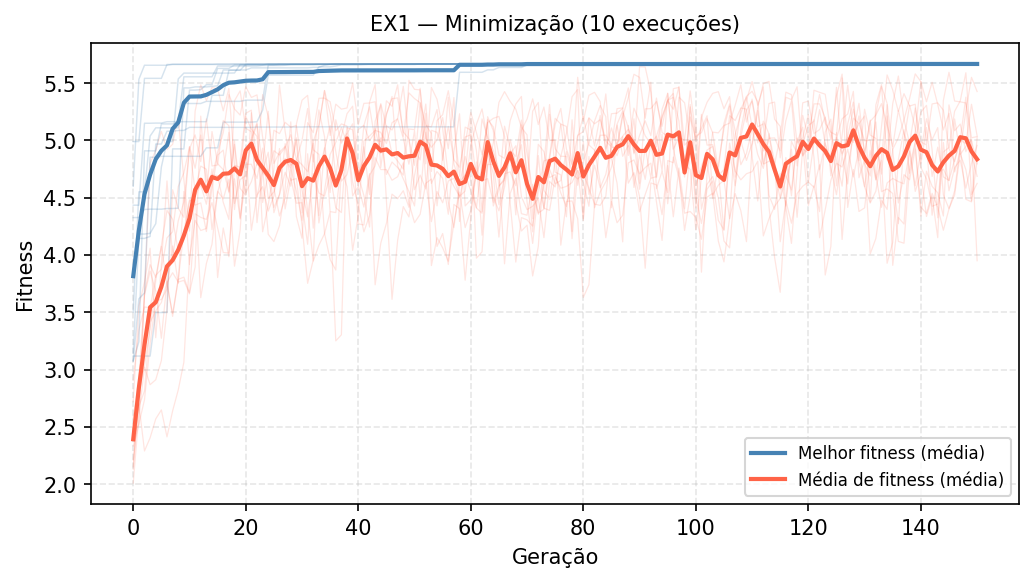
\includegraphics[width=\columnwidth]{ex1_min_conv.png}
  \caption{Convergência do EX1 --- Minimização (10 execuções).}
  \label{fig:ex1min}
\end{figure}

\subsection{Experimento 2: Problema dos Rádios}

O segundo experimento consiste em um problema de programação linear inteira com duas
variáveis de decisão: $ST$ (rádios Standard) e $LX$ (rádios Luxo).

\textbf{Função objetivo:}
\begin{equation}
  FO = 30 \cdot ST + 40 \cdot LX
  \label{eq:fo2}
\end{equation}

\textbf{Restrição principal:}
\begin{equation}
  ST + 2 \cdot LX \le 40
  \label{eq:restricao}
\end{equation}

\textbf{Domínios:} $0 \le ST \le 24$ e $0 \le LX \le 16$.

\textbf{Representação.} O cromossomo binário possui 10~bits: os 5~primeiros codificam $ST$
e os 5~últimos codificam $LX$. Cada bloco de 5~bits é convertido para decimal e ajustado
ao intervalo correspondente pela Equação~\ref{eq:scale}. Como os domínios são inteiros, os
valores obtidos são arredondados. Com 5~bits por variável, têm-se $2^5 = 32$ valores
distintos por variável.

\textbf{Função de \textit{fitness}.} A restrição é tratada por penalização. A violação
normalizada é:
\begin{equation}
  H_n = \max\!\left(0,\; \frac{ST + 2 \cdot LX - 40}{16}\right)
  \label{eq:hn}
\end{equation}

A função objetivo normalizada e a \textit{fitness} são:
\begin{equation}
  FO_n = \frac{30 \cdot ST + 40 \cdot LX}{1360}, \qquad
  \mathit{fit} = FO_n - H_n
  \label{eq:fit2}
\end{equation}

O coeficiente de penalidade $r = -1$ desestimula soluções que violam a restrição,
conduzindo o algoritmo a soluções viáveis.

\textbf{Configuração.} Parâmetros: $N = 10$, $G = 150$, $p_c = 0{,}8$, $p_m = 0{,}05$,
\textit{crossover} de um ponto e elitismo ativado.

\textbf{Resultados.}
A Tabela~\ref{tab:ex2} apresenta os resultados das 10~execuções.

\begin{table}[H]
\centering
\caption{Resultados do problema dos rádios (10 execuções).}
\label{tab:ex2}
\small
\begin{tabular}{@{}crrrrrr@{}}
\toprule
Exec. & $ST$ & $LX$ & $FO$ & Infr. & \textit{Fitness} \\
\midrule
1  & 24 & 8 & 1040 & 0 & 0,7647 \\
2  & 24 & 8 & 1040 & 0 & 0,7647 \\
3  & 24 & 8 & 1040 & 0 & 0,7647 \\
4  & 24 & 8 & 1040 & 0 & 0,7647 \\
5  & 24 & 8 & 1040 & 0 & 0,7647 \\
6  & 24 & 8 & 1040 & 0 & 0,7647 \\
7  & 24 & 8 & 1040 & 0 & 0,7647 \\
8  & 24 & 8 & 1040 & 0 & 0,7647 \\
9  & 24 & 8 & 1040 & 0 & 0,7647 \\
10 & 24 & 8 & 1040 & 0 & 0,7647 \\
\midrule
\multicolumn{4}{l}{\textbf{Média}} & & 0,7647 \\
\multicolumn{4}{l}{\textbf{Desv. Pad.}} & & 0,0000 \\
\bottomrule
\end{tabular}
\end{table}

A Figura~\ref{fig:ex2} apresenta as curvas de convergência das 10~execuções.

\begin{figure}[H]
  \centering
  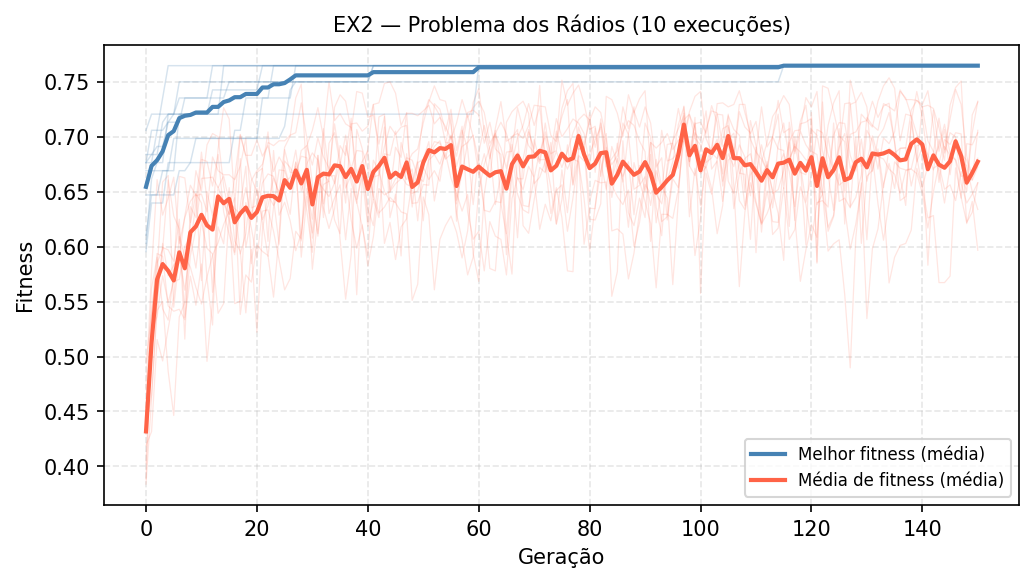
\includegraphics[width=\columnwidth]{ex2_conv.png}
  \caption{Convergência do EX2 --- Problema dos rádios (10 execuções).}
  \label{fig:ex2}
\end{figure}

\subsection{Experimento 3: Problema 3-SAT}

O terceiro experimento consiste em uma instância 3-SAT com 100~variáveis booleanas e
430~cláusulas, carregada a partir de um arquivo no formato DIMACS CNF. Cada cláusula
possui 3~literais, que podem representar variáveis na forma positiva ($x_i$) ou
negada ($\neg x_i$). O objetivo é encontrar uma atribuição de valores booleanos que
satisfaça o maior número possível de cláusulas.

\textbf{Representação.} O cromossomo é uma sequência de 100~bits, onde o bit~$i$
representa o valor lógico da variável~$x_i$ (0~= falso, 1~= verdadeiro). Um literal
positivo $x_i$ é satisfeito quando o bit correspondente é~1; um literal negativo $\neg x_i$
é satisfeito quando o bit correspondente é~0. Uma cláusula (disjunção de 3~literais) é
satisfeita quando ao menos um de seus literais é satisfeito.

\textbf{Função de \textit{fitness}.} A função objetivo é o número de cláusulas satisfeitas
pelo cromossomo:
\begin{equation}
  FO = \#\{\text{cláusulas satisfeitas}\}, \qquad
  \mathit{fit} = \frac{FO}{430}
  \label{eq:fit3}
\end{equation}

O valor de \textit{fitness} varia em $[0, 1]$, sendo~1 o máximo possível (todas as
cláusulas satisfeitas).

\textbf{Configuração.} Parâmetros: $N = 30$, $G = 2000$, $p_c = 0{,}8$, $p_m = 0{,}01$,
\textit{crossover} de um ponto e elitismo ativado.

\textbf{Resultados.}
A Tabela~\ref{tab:ex3} apresenta os resultados das 10~execuções.

\begin{table}[H]
\centering
\caption{Resultados do problema 3-SAT (10 execuções).}
\label{tab:ex3}
\small
\begin{tabular}{@{}crrr@{}}
\toprule
Exec. & Cl. sat. & Cl. não sat. & \textit{Fitness} \\
\midrule
1  & 425 &  5 & 0,988372 \\
2  & 423 &  7 & 0,983721 \\
3  & 424 &  6 & 0,986047 \\
4  & 419 & 11 & 0,974419 \\
5  & 423 &  7 & 0,983721 \\
6  & 425 &  5 & 0,988372 \\
7  & 427 &  3 & 0,993023 \\
8  & 421 &  9 & 0,979070 \\
9  & 423 &  7 & 0,983721 \\
10 & 423 &  7 & 0,983721 \\
\midrule
\multicolumn{2}{l}{\textbf{Média}} & & 0,984419 \\
\multicolumn{2}{l}{\textbf{Desv. Pad.}} & & 0,004884 \\
\bottomrule
\end{tabular}
\end{table}

A Figura~\ref{fig:ex3} apresenta as curvas de convergência das 10~execuções para o
problema 3-SAT.

\begin{figure}[H]
  \centering
  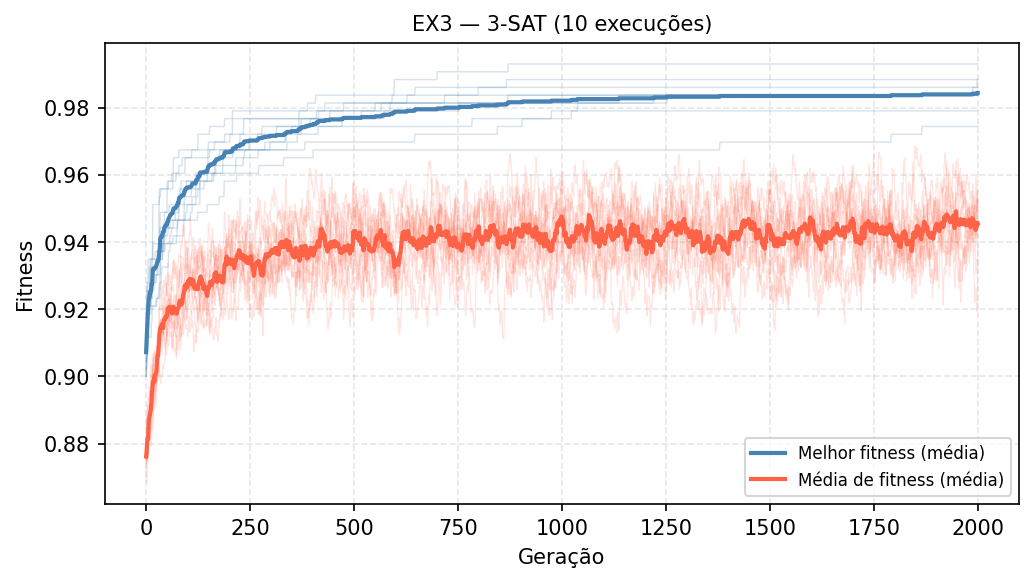
\includegraphics[width=\columnwidth]{ex3_conv.png}
  \caption{Convergência do EX3 --- 3-SAT (10 execuções).}
  \label{fig:ex3}
\end{figure}

\subsection{Box-Plots Comparativos}

A Figura~\ref{fig:boxplot} apresenta os box-plots do melhor \textit{fitness} final de cada
execução para todos os experimentos. A visualização permite comparar a variabilidade e a
tendência central dos resultados entre os diferentes problemas.

\begin{figure}[H]
  \centering
  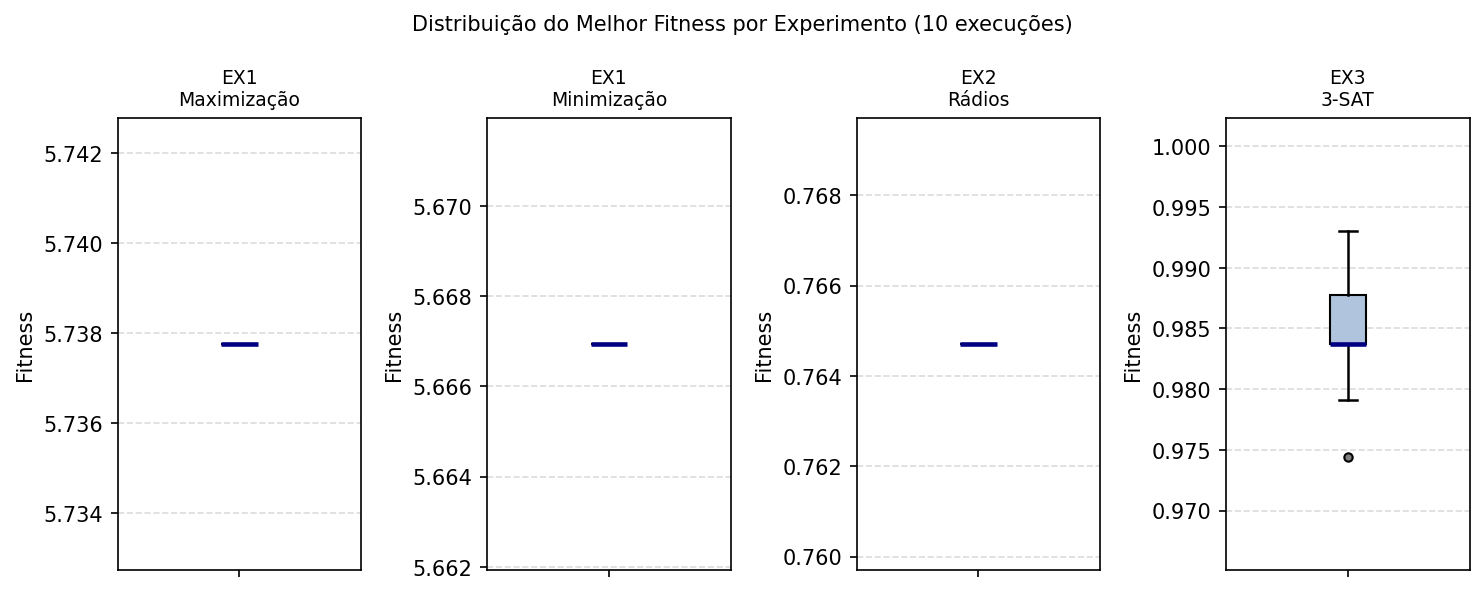
\includegraphics[width=\columnwidth]{boxplot_geral.png}
  \caption{Distribuição do melhor \textit{fitness} por experimento (10 execuções).}
  \label{fig:boxplot}
\end{figure}

% ------------------------------------------------------------------
\section{Análise dos Resultados}
% ------------------------------------------------------------------

A realização de 10~execuções independentes com os mesmos parâmetros teve como objetivo
avaliar a estabilidade da ferramenta diante da aleatoriedade característica dos AGs.

\textbf{EX1 --- Maximização.}
Todas as execuções convergiram para a mesma região do espaço de busca, com $x \approx
1{,}8904$ e $f(x) \approx 1{,}7378$. O desvio padrão do \textit{fitness} final foi de
apenas~$6 \times 10^{-6}$, evidenciando estabilidade muito elevada. O valor encontrado
corresponde ao máximo local proeminente da função no domínio $[-2, 2]$, onde o efeito
combinado do crescimento cúbico e do cosseno gera um pico acentuado em $x \approx 1{,}89$.

As curvas de convergência (Figura~\ref{fig:ex1max}) mostram que o melhor
\textit{fitness} cresce rapidamente nas primeiras~50 gerações e se estabiliza
completamente antes da geração~100. Esse padrão é coerente com o uso de elitismo, que
garante a preservação do melhor indivíduo encontrado. A média de \textit{fitness} oscila
ao longo de todas as gerações, indicando que a população continua sendo modificada pelos
operadores genéticos, mantendo diversidade.

\textbf{EX1 --- Minimização.}
A minimização apresentou estabilidade ainda mais elevada: todas as 10~execuções
convergiram exatamente para $x = -2{,}0000$, com $f(x) = -3{,}6669$ e desvio padrão
nulo. O resultado corresponde ao extremo inferior do domínio avaliado, onde a função
atinge seu valor mínimo. A alta consistência indica que a codificação binária com 16~bits
oferece resolução suficiente para que o algoritmo localize esse ponto de forma inequívoca.

As curvas de convergência (Figura~\ref{fig:ex1min}) apresentam padrão semelhante ao da
maximização: subida rápida nas primeiras gerações, seguida de estabilização completa do
melhor indivíduo. A média de \textit{fitness} oscila mais do que no caso da maximização,
pois os operadores genéticos continuam explorando soluções subótimas na vizinhança do
mínimo.

\textbf{EX2 --- Problema dos Rádios.}
Todas as 10~execuções convergiram para a mesma solução fenotípica: $ST = 24$ e
$LX = 8$. A solução respeita exatamente a restrição principal, pois:
$ST + 2 \cdot LX = 24 + 2 \times 8 = 40 \le 40$. O valor da função objetivo foi
$FO = 30 \times 24 + 40 \times 8 = 1040$, com $H_n = 0$ e \textit{fitness} igual
a $1040/1360 \approx 0{,}7647$. O desvio padrão entre execuções foi nulo.

Esse resultado sugere que a modelagem por penalização foi adequada: o coeficiente
$r = -1$ cria um incentivo suficientemente forte para evitar soluções inviáveis, ao mesmo
tempo que favorece soluções com alto valor de função objetivo. A convergência rápida
(antes de 50~gerações, em média) indica que o espaço de busca de 10~bits é relativamente
pequeno ($2^{10} = 1024$ soluções possíveis) e o AG o explora eficientemente.

\textbf{EX3 --- 3-SAT.}
O problema 3-SAT apresentou maior variabilidade do que os experimentos anteriores,
conforme esperado dado o tamanho do espaço de busca ($2^{100}$ possíveis atribuições).
O número de cláusulas satisfeitas variou entre~419 e~427 (de um total de~430), com média
de $423{,}6$ e desvio padrão de~$2{,}1$ cláusulas. A média do \textit{fitness} final foi
$0{,}9844$ com desvio padrão de~$0{,}0049$.

Nenhuma execução encontrou uma solução que satisfizesse todas as 430~cláusulas. A melhor
execução satisfez 427~cláusulas ($\approx 99{,}3\%$ do total), deixando apenas~3~cláusulas
insatisfeitas. Esse resultado indica alta qualidade das soluções encontradas, mesmo em um
domínio combinatório de dimensão extremamente elevada.

As curvas de convergência (Figura~\ref{fig:ex3}) mostram crescimento mais gradual do
melhor \textit{fitness} em comparação aos experimentos anteriores. O melhor \textit{fitness}
tende a estabilizar antes do término das 2000~gerações, sugerindo que o algoritmo encontrou
regiões promissoras do espaço de busca, mas teve dificuldade para melhorar os últimos valores.
Isso se deve à interdependência entre as cláusulas: uma alteração de bit pode satisfazer
novas cláusulas e, simultaneamente, tornar outras insatisfeitas.

\textbf{Comparação entre experimentos.}
O box-plot da Figura~\ref{fig:boxplot} ilustra claramente as diferenças de variabilidade:
os experimentos EX1~Min e EX2 não apresentam variação (caixas degeneradas em um único
ponto), enquanto EX1~Max apresenta variação mínima e EX3 apresenta variação perceptível,
porém pequena em termos absolutos. Essa análise confirma que problemas de menor dimensão
e espaço de busca mais estruturado levam a uma convergência mais consistente.

% ------------------------------------------------------------------
\section{Conclusões e Trabalhos Futuros}
% ------------------------------------------------------------------

Este trabalho apresentou o desenvolvimento de uma ferramenta genérica para execução de
Algoritmos Genéticos em Python, avaliada em três problemas com características distintas.
A ferramenta demonstrou capacidade de produzir soluções de alta qualidade e consistência,
com a mesma estrutura evolutiva adaptada a domínios diferentes por meio de funções de
\textit{fitness} específicas.

Os resultados experimentais confirmam que:
(i)~a ferramenta encontrou soluções próximas ao ótimo global em todos os problemas
testados;
(ii)~o uso de elitismo garante a preservação de boas soluções entre gerações;
(iii)~a penalização por violação de restrição foi eficaz no EX2;
(iv)~a variabilidade entre execuções aumenta com a complexidade do problema, mas permanece
controlada pelo elitismo.

Como trabalhos futuros, propõe-se: (a)~implementar novos métodos de seleção, como
torneio e \textit{ranking}; (b)~completar os operadores de mutação e \textit{crossover}
para representações inteiras e reais; (c)~avaliar critérios de parada adaptativos baseados
na convergência da média populacional; e (d)~paralelizar o cálculo de \textit{fitness}
para reduzir o tempo de execução em problemas com avaliação custosa.

\bibliographystyle{sbc}
\begin{thebibliography}{99}

\bibitem{vonzuben2000}
Von Zuben, F.~J. (2000).
\newblock Computação evolutiva: uma abordagem pragmática.
\newblock Tutorial, FEEC/Unicamp.

\bibitem{tutorialspoint2016}
Tutorials Point (2016).
\newblock \textit{Genetic Algorithms Tutorial}.
\newblock Disponível em: \url{https://www.tutorialspoint.com/genetic_algorithms/}

\bibitem{goldberg1989}
Goldberg, D.~E. (1989).
\newblock \textit{Genetic Algorithms in Search, Optimization, and Machine Learning}.
\newblock Addison-Wesley.

\bibitem{mitchell1998}
Mitchell, M. (1998).
\newblock \textit{An Introduction to Genetic Algorithms}.
\newblock MIT Press.

\end{thebibliography}

\end{document}
